<%= heading2 %>{Abbildungen}

<%- bexample %>
<%- Cref %>{fig:label} zeigt etwas Interessantes

\begin{figure}
  \centering
  Füge deine Abbildung hier ein.
  \caption{Bildunterschrift.}
  \label{fig:label}
\end{figure}
<%- eexample %>

Fotos im JPEG- oder PNG-Format werden genauso eingebunden, wie <%- cref %>{fig:jpg} zeigt.

<%- bexample %>
\begin{figure}
  \centering
  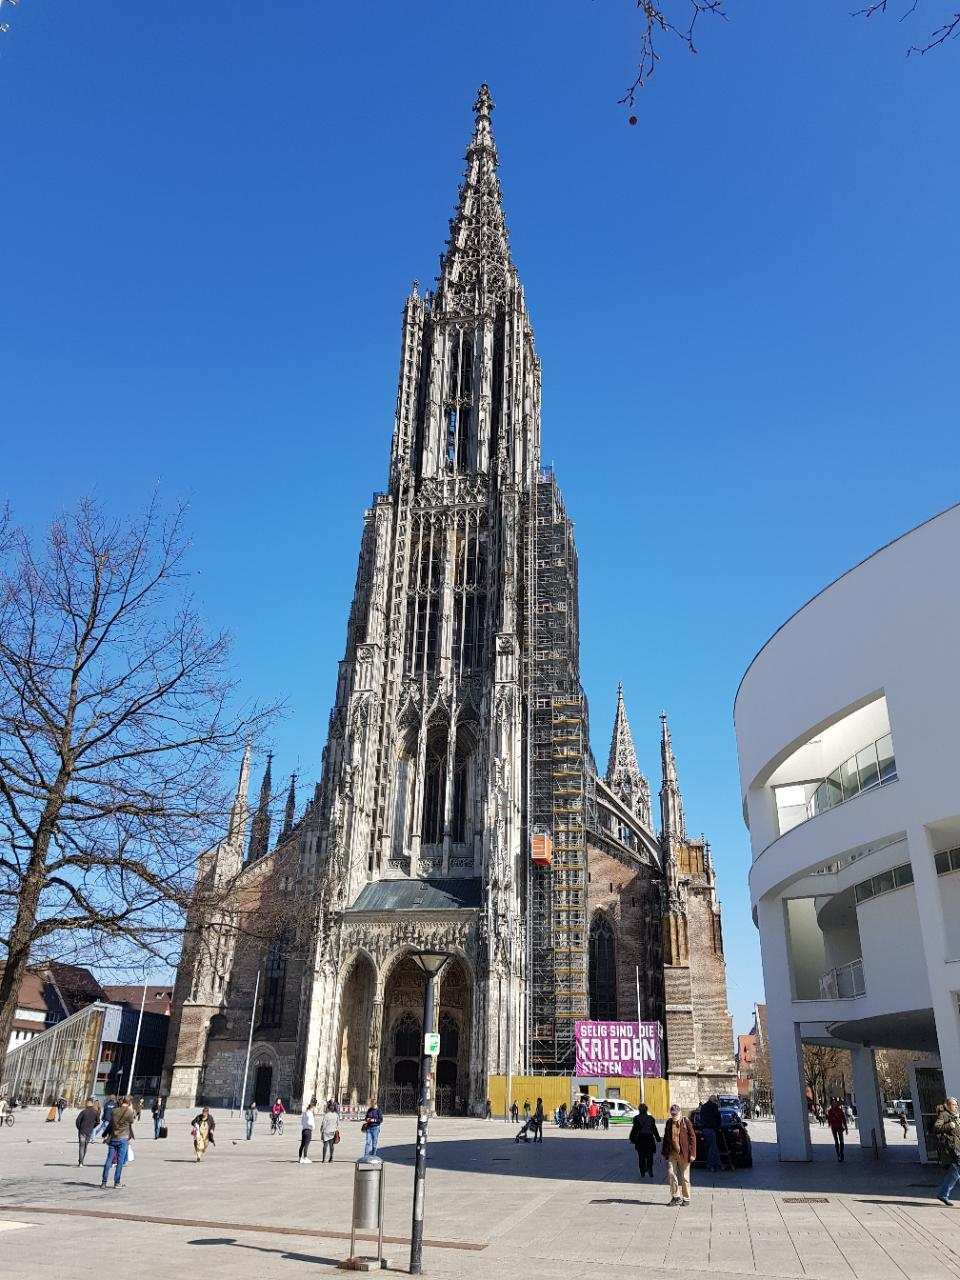
\includegraphics[width=.5\linewidth]{figures/ulm-minster.jpg}
  \caption{Ulmer Münster. Foto: wkrauth, CC0, via Wikimedia Commons.}
  \label{fig:jpg}
\end{figure}
<%- eexample %>
<%- include('floatflt.example.en.tex', this); -%>
<% if (documentclass == 'ieee') { -%>

One can span a figure across multiple columns by using \verb+\begin{figure*}+.
See <%- cref %>{fig:16x9} as an example.

<%- bexample %>
\begin{figure*}
  \centering
  % note that \textwidth is used instead of \linewidth
  % This ensures that the graphics width is 60% of the "page" (text block), and not just 60% of the current text column
  % See https://tex.stackexchange.com/a/17085/9075 for details
  \includegraphics[width=.6\textwidth]{example-image-16x9}
  \caption{16x9 Figure}
  \label{fig:16x9}
\end{figure*}
<%- eexample %>

<% } -%>
